% Author: Pavol Loffay
% Project: Master thesis - Hawkular alrt prediction
% Date 20.2.2015

\documentclass[12pt,oneside]{fithesis2}
% Packages
\usepackage[english]{babel}       % Multilingual support
\usepackage[utf8]{inputenc}       % UTF-8 encoding
\usepackage[T1]{fontenc}          % T1 font encoding
\usepackage[scaled=0.86]{berasans}
\usepackage[scaled=1.03]{inconsolata}
\usepackage[plainpages = false,pdfpagelabels]{hyperref}
\usepackage{blindtext}            % Lorem ipsum generator


\thesistitle{Alert prediction in metric data based on machine learning methods} % enter thesis title  
\thesissubtitle{Master thesis}  
\thesisstudent{Pavol Loffay}    % name of the author  
\thesiswoman{false}          % defines author’s gender  
\thesisfaculty{fi}  
\thesisyear{spring 2016}  
\thesisadvisor{RNDr. Adam Rambousek} % fill in advisor’s name  
\thesislang{en}                 % thesis is in English  

\begin{document}
\FrontMatter                    % The front matter
\ThesisTitlePage                % The title page
\begin{ThesisDeclaration}       % The declaration
  \DeclarationText
  \AdvisorName
\end{ThesisDeclaration}

\begin{ThesisThanks}            % The acknowledgements (optional)
  I would like to thank my supervisor Jiri Kremser, family and 
  the people from Hawkular team.
\end{ThesisThanks}

\begin{ThesisAbstract}          % The abstract
  The aim of the master thesis was to develop a module for open source monitoring
  and management platform Hawkular. This module is responsible for predicting
  alerts based on time series. 
\end{ThesisAbstract}

\begin{ThesisKeyWords}          % The keywords
  Time Series, Hawkular, Alert Prediction, ARIMA, Apache Spark.
\end{ThesisKeyWords}

\tableofcontents                % The table of contents
%   \listoftables                   % The list of tables (optional)
%   \listoffigures                  % The list of figures (optional)

\MainMatter                     % The main matter
% Author: Pavol Loffay
% Project: Master thesis - Hawkular alert prediction
% Date 20.2.2015

\chapter{Introduction} 
Alert prediction is very important because it can predict critical states of a system in
advance. It gives system administrators powerful feature to reduce downtime and
of course ability to use all of the available resources in the system. 

\section{Context}
Implementation part of the master thesis is developed as part of the project
Hawkular\footnote{Available at \url{http://www.hawkular.org}}. 
Therefore application architecture and used technologies had to fit 
in the overall project architecture.

Hawkular is open source monitoring and management platform mainly
developed by company Red Hat. It is successor of very successful RHQ
project\footnote{Available at \url{https://rhq-project.github.io/rhq/}}.
This application is designed to monitor Java middleware 
like Wildfly and Apache Tomcat. For instance it can monitor heap usage, web
sessions, used data sources etc.

\section{Goals}
The main goal of the application is to provide users with reliable predictions
of alerts for the set of collected metrics. Displaying of forecast is also very
important and should be available in the user interface. This feature can help 
system administrators react on events like running out of memory well
in advance.

%%%%%%%%%%%%%%%%%%%%%%%%%%%%%%%%%%%%%%%%%%%%%%%%%%%%%%%%%%%%%%%%%%% 
\chapter{Time Series Analysis}
In this chapter are discussed various approaches for forecasting time series and
also relevant theory which is helpful for understanding them.
Methods are ordered from simpler to more complex. 

In the early part of the thesis
development system R was used to quickly show the results of forecasting and
better understanding metric data by plotting them. 

Firstly it is important to define time series; it is sequence of observations
$ s_t \in \mathbb{R} $ usually ordered in time. In this thesis are used only
discrete univariate time series. 

Forecasting is a process of making prediction of the future based 
on the past. In other words forecasting is possible because  
future depends on the past or analogously because there is a relationship
between the future and the past. However this relation is not deterministic and 
can be hardly written in an analytical form.


There are two forecasting types: qualitative and quantitative.
Qualitative methods are mainly based on the opinion of the subject and are used 
when past data are not available, hence not suitable for this project. 
When there are past data available quantitative forecasting methods can be used. 

\section{Simple quantitative methods}

There are three simple forecasting methods:
\begin{itemize}
    \item Average method\,--\,forecasts are equal to the value of the mean of
        historical data 
        $$ \hat{y}_{T+h|T} = \overline{y} = (y_{1}+ \dots + y_{T}) / T $$
    \item Na\"{i}ve method\,--\,forecasts are equal to the last observed value
        $$ \hat{y}_{T+h|T} = y_{T} $$ 
    \item Drift method\,--\,variation of na\"{i}ve method which allow the
        forecasts to increase or decrease over time
        $$ \hat{y}_{T+h|T} = y_{T} + \frac{h}{T-1} \sum_{t=2}^T{y_{t} - y_{t-1}} = 
        y_{T} + h(\frac{y_{T}-y_{1}}{T-1}) $$
\end{itemize}
There in also seasonal variant of na\"{i}ve method. This method is suitable only
for highly seasonal data. Forecast is simply equal to last observed value from
the previous season.

\section{Time series decomposition}
In the time series can be seen various patterns. It is crucial to categorize
some of them. These patters are useful to split into several components 
each representing one of the underlying categories of pattern. This approach is
done when modelling 

Basic patterns are trend, seasonality, cycle and irregular component. 

\begin{itemize}
    \item \textbf{Trend $ T_{t} $}\,--\,exists if there is long term increase or decrease over
        time. Can be linear or nonlinear (e.g. exponential growth)
    \item \textbf{Seasonal $ S_{t} $}\,--\,exists when a series is influenced by seasonal factors.
        Seasonality is always of fixed and known period.
    \item \textbf{Cyclic $ C_{t} $}\,--\,exists it there long term wave\,--\,like patterns.
        Unlike trend waves are not of fixed period.
    \item \textbf{Irregular $ N_{t} $}\,--\,unpredictable random value
\end{itemize}

Decomposition can be in many forms for instance two of them are additive or multiplicative model.

\begin{eqnarray}
    y_{t} = T_{t} + S_{t} + C_{t} + N_{t} \\
    y_{t} = T_{t} \times S_{t} \times C_{t} \times N_{t} 
\end{eqnarray}

Seasonality can be modelled by using \emph{Dummy} variables.



\section{Averaging and smoothing models}
\subsection{Moving Average Smoothing}
This model can eliminate some randomness in the data 
\subsection{Exponential Smoothing}
The concept behind simple exponential smoothing is to attach 
larger weights to most recent observations than to observations from distant
past. Forecasts are calculated using weighted averages where the weights 
decrease exponentially as observations come from further in the past.
In other words smaller weights are associated to older observations.

$$ \hat{y}_{T+1|T} = \alpha y_{T} + \alpha(1-\alpha)y_{T-1} +
    \alpha(1-\alpha)^2 y_{T-2} +\dots $$
Smoothing parameter is $ 0 \leq \alpha \leq 1 $. Note, if $\alpha = 1$ then 
$\hat{y}_{T+1|T} = y_{T}$ so forecasts are equal to the na\"{i}ve method.
If the $\alpha $ is smaller more weight is given to observations from distance
in past. 

Simple exponential smoothing has flat forecast function, that means all forecast
all the same. Smoothing can be generally used as technique to separate signal and noise.
This method is useful if a series doesn't contain any trend.

\subsubsection{Holt's Liner Trend Method}
Simple exponential smoothing can be extended to allow forecasting of data with a trend. 
This was done by Charles C. Holt in 1957. This method is slightly more complicated than 
original one without trend. In order to add trend component another equation is added. 
$$ \hat{y}_{t+h|t} = l_{t} + hb_{t} $$
$$ l_t = \alpha y_t + (1 - \alpha) (l_{t-1} + b_{t-1})$$
$$ b_t = \beta^{*} (l_t - l_{t-1}) + (1 - \beta^{*})b_{t-1} $$

Where $b_t$ denotes slope of the time series and $l_t$ level. There is also a new parameter $\beta$
\,--\,smoothing parameter of the slope. It's rage is equal to $\alpha$, so $\alpha,\beta
\in \interval[{0,1}]$. 
\section{Linear Regression}

\section{White noise}
\section{Stationarity}

\section{Box\,--\,Jenkins Methods}

%%%%%%%%%%%%%%%%%%%%%%%%%%%%%%%%%%%%%%%%%%%%%%%%%%%%%%%%%%%%%%%%%%% 
\chapter{Used Forecasting Techniques}
In the previous chapter several methods for forecasting were discussed, however
in our system only a few of them were selected and implemented.

\section{Metrics in Hawkular}
In Hawkular there are three types of metrics: gauge, counter and availability. 
All of them are univariate metrics of structure $ \{timestamp, value\} $.

%%%%%%%%%%%%%%%%%%%%%%%%%%%%%%%%%%%%%%%%%%%%%%%%%%%%%%%%%%%%%%%%%%% 
\chapter{Design and Implementation}
\section{Architecture}
As was sad module was developed as module of Hawkular project, therefore was
important to follow architecture of whole application. Alert prediction module
was developed as standalone web application in Java language. Communication with
other modules was accomplished through Java Message Service and REST calls. 

Following diagram \ref{img_arch} shows how this module fits to Hawkular application.
Almost all of the modules are developed separately and can work without each
other. However this module is depended on metrics module and alerts. 
\begin{figure}[H]
    \begin{center}
        %TODO change to UML component diagram
        \scalebox{0.5}{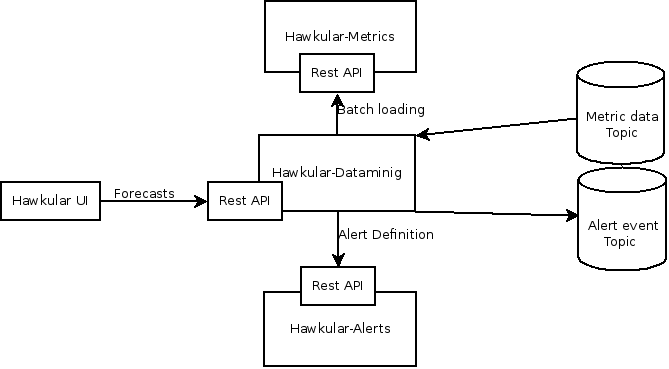
\includegraphics{img/architecture.png}} 
        \caption{Architecture}
        \label{img_arch}
    \end{center}
\end{figure}

%%%%%%%%%%%%%%%%%%%%%%%%%%%%%%%%%%%%%%%%%%%%%%%%%%%%%%%%%%%%%%%%%%% 
\chapter{Evaluation}
%%%%%%%%%%%%%%%%%%%%%%%%%%%%%%%%%%%%%%%%%%%%%%%%%%%%%%%%%%%%%%%%%%% 
\chapter{Conclusion}
\cite{rfc_owamp} %TODO remove


    
% Bibliography goes here
% Index goes here (optional)
\bibliographystyle{czechiso} % sets plain bibliography style  
\bibliography{bibliography}     % BibTeX database file 
\end{document}

